Before analysis, data must be preproccessed in order to standardize image properties and reduce the likelyhood of errors in classififcation. A collection of scripts were run on each of the maps prior to classification. Images were rotated and scaled and Blue lines were removed using colour filter masks. Colour information was also removed from the images bringing them to a black and white only state. Each cell was scaled to a standard 75 by 75 pixels and seperated from the map as a whole such that each cell contrains only a single symbol.

\begin{figure}[h]
    \begin{center}
    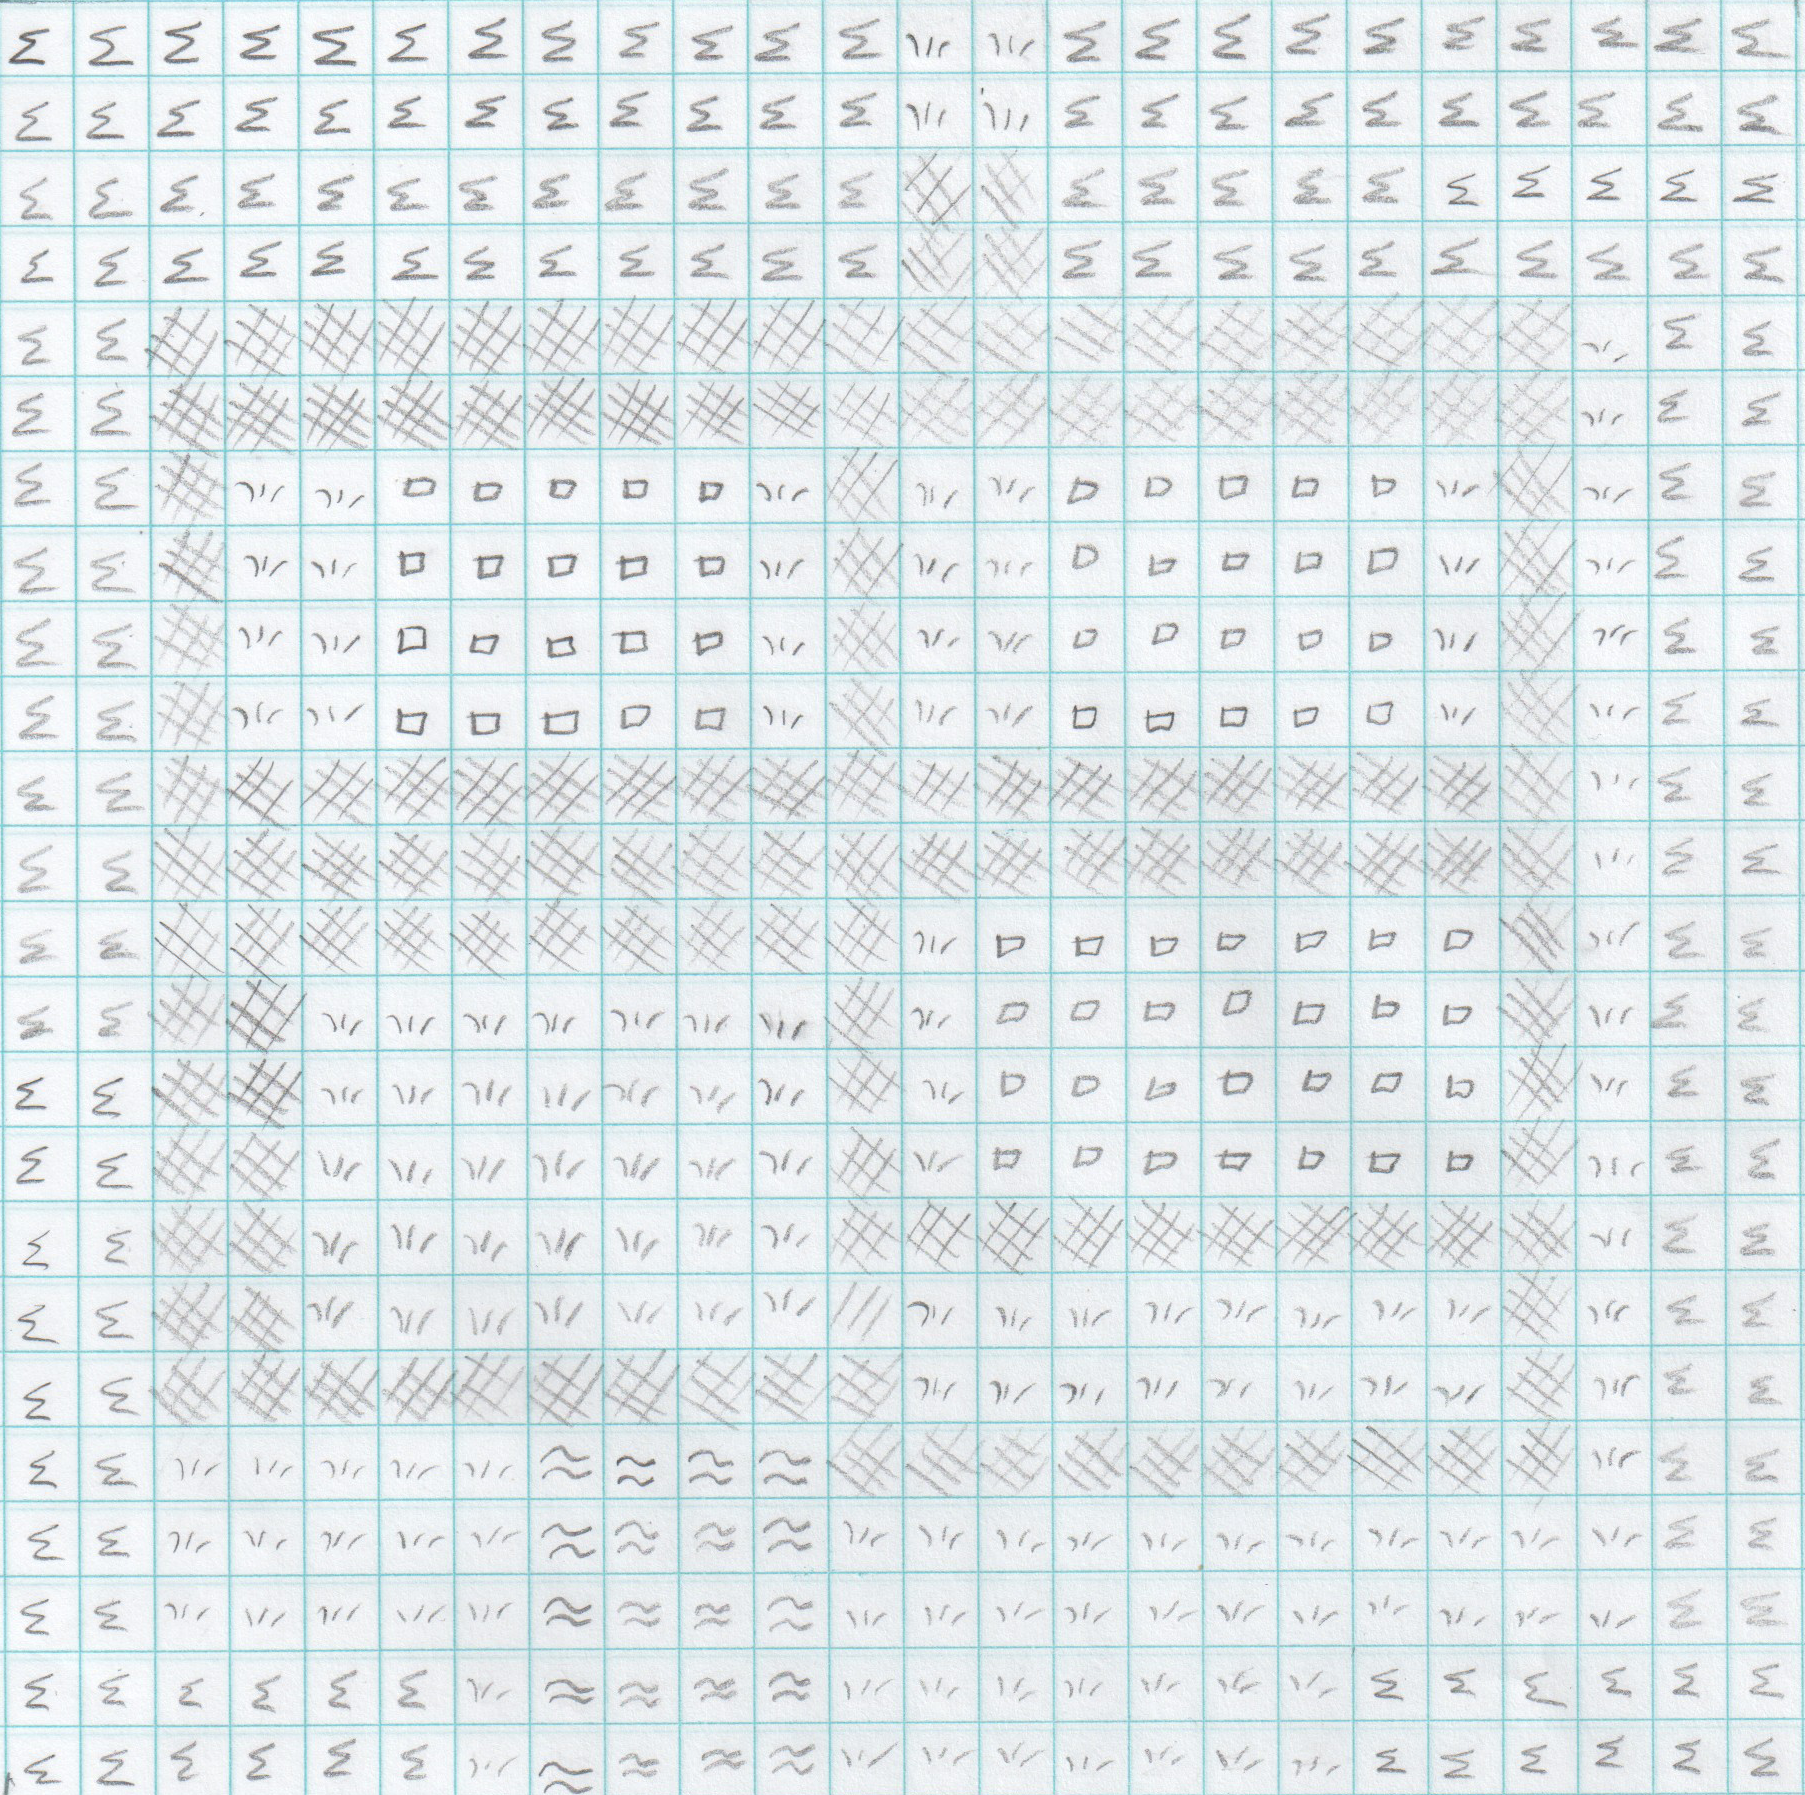
\includegraphics[width=7.5cm, height=7.5cm]{preprocessing-initial}
    \includegraphics[width=7.5cm, height=7.5cm]{preprocessing-final}
    \caption{Image before preprocessing and image after preprocessing. Notice
        that the contrast has increased and the blue lines have been partially
        removed}
    \end{center}
\end{figure}
